% Beamer template
% Author: Ozgur Taylan TURAN
% Delft University of Technology

\documentclass[aspectratio=169]{beamer}
% PACKAGES
\usepackage[english]{babel}
\usepackage{graphicx}
\usepackage{animate}
%\usepackage{calc}
\usepackage{calligra}
\usepackage[absolute,overlay]{textpos}
\usepackage[T1]{fontenc}
%\usefonttheme{serif}
\usefonttheme{professionalfonts}
\usepackage{amsmath}
\usepackage{palatino}
\usepackage{mathpazo}
\usepackage{graphicx}
%\usepackage{subfig}
\usepackage{tikz}
\usetikzlibrary{shapes,arrows}
\usepackage{xcolor}
\usepackage[T1]{fontenc}
%\usefonttheme{serif}
%\usepackage{titling}
\usepackage{graphicx}
%\usepackage{subfig}
%\usepackage{tikz}
%\usetikzlibrary{shapes,arrows}
\usepackage{mathtools}
\usepackage{cancel}
% CUSTOM PACKAGES
\usepackage{/home/taylanot/texmf/tex/beamerthemetot}
\input{/home/taylanot/texmf/presentation/tune.tex}

% COVER PAGE INFO   
\newcommand{\mytitle}{\color{White}\huge{\textbf{Coffee Talk \#6}}}
\newcommand{\mysubtitle}{\color{Pink}\Large{\textbf{DeepONet:Learning nonlinear operators for identifying differential equations based on the universal approximation theorem of operators}}}
\newcommand{\myauthor}{\color{White}\textcalligra{\LARGE Ozgur Taylan Turan}}
\newcommand{\authorlabel}{\small O.T. Turan}
\author{\authorlabel}


\begin{document}
% COVER PAGE

{
\def\beamer@entrycode{\vspace*{-\headheight}}
\setbeamertemplate{frametitle}[default][center]
\setbeamertemplate{navigation symbols}{}
\usebackgroundtemplate{
\includegraphics[width=\paperwidth,height=\paperheight]{cover/coverart.pdf}}

\begin{frame}[plain] 

\begin{minipage}{\textwidth}
	\centering{\mytitle} \\
	%\vspace{1cm}
	%\centering{\mysubtitle} \\
	\vspace{1cm}
	\centering{\color{White}November 15, 2021} \\
	\vspace{1cm}
	\centering{\myauthor}\\
\end{minipage}
\end{frame}
}


\begin{frame}
  \centering
  \mysubtitle\cite{lu2021a}
\end{frame}

\begin{frame}{Why this paper?}
  \centering
  \begin{itemize}
    \item Badly written, but has an interesting problem to tackle!
  \end{itemize}
\end{frame}


\begin{frame}{Preliminary Info}
  \begin{minipage}{0.5\textwidth}
    \color{Pink}{Function}\color{Black}
    \centering

    $f:=\mathcal{V}\to\mathcal{V}$
  \end{minipage}%
  \begin{minipage}{0.5\textwidth}
    \color{Pink}{Operator}\color{Black}
    \centering

    $G:=\mathcal{F}\to\mathcal{V}$
  \end{minipage}

  \centering

  $\mathcal{V}$: Vector Space

  $\mathcal{F}$: Function Space

  \begin{itemize}
    \item $G(u):=s(x)$, where $u$ is a function of $x$ 
    \item At a location $y$ the operator evaluation is given by $G(u)(y):=s(y)$
  \end{itemize}
\end{frame}

\begin{frame}{Universal Approximation Theorems}

  \begin{minipage}{0.5\textwidth}
    \color{Pink}{Universal Approximation Theorem for Function}\color{Black}
    \centering

    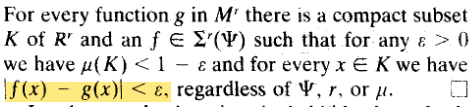
\includegraphics[width=0.8\textwidth]{Figures/fun.png}\cite{hornik1989}
  \end{minipage}%
  \begin{minipage}{0.5\textwidth}
    \color{Pink}{Universal Approximation Theorem for Operator}\color{Black}
    \centering

    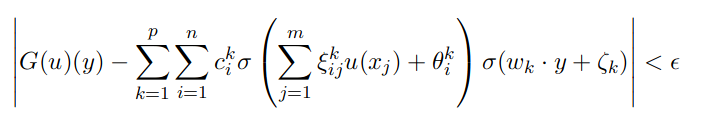
\includegraphics[width=\textwidth]{Figures/op.png}\cite{chen1995}

  \end{minipage}

\end{frame}

\begin{frame}{What does it look like?}
  \centering
  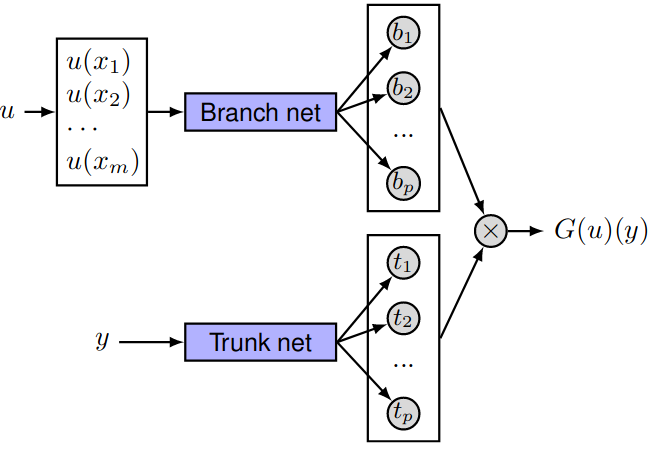
\includegraphics[width=0.65\textwidth]{Figures/pic.png}
\end{frame}

\begin{frame}{What does it look like?}
  \begin{minipage}{0.5\textwidth}
    \centering
    Try to find the following operator:

    $G:=u(x)\to s(x)=\int_0^x u(\tau)d\tau$

  \end{minipage}%
  \begin{minipage}{0.5\textwidth}
    \centering
    Procedure:
    \begin{itemize}
      \item \textbf{Sample $(u_k)_{k=1}^{p}$ from Gaussian  Random Field at locations $(x_i)_{i=1}^m$}
      \item For every function obtain some of the exact outputs at $y$ of function $G(u)$
      \item Train with the given structure and selected hyper-parameters 
    \end{itemize}
  \end{minipage}
\end{frame}

\begin{frame}{Training Curve}
  \centering
  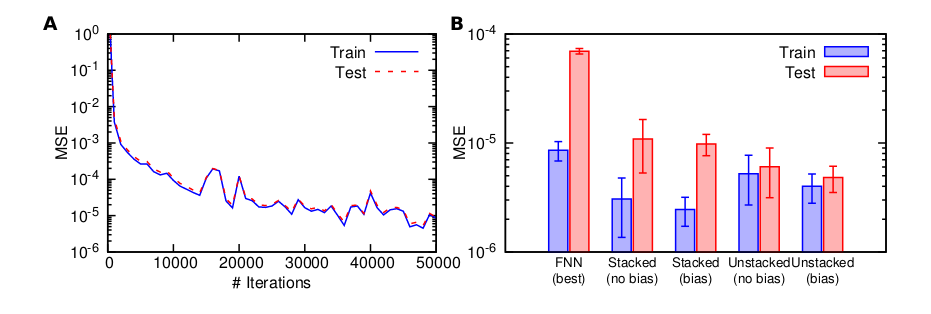
\includegraphics[width=0.85\textwidth]{Figures/res.png}
\end{frame}

\begin{frame}{No Results?}

  \color{Pink} Please, check the paper for extensive examples!

\end{frame}

\begin{frame}{Why is this a cool idea?}
  \begin{itemize}
    \item Solving ODEs/SODEs can be challenging...
    \item Previous data usage for fast prediction for dynamical systems
    \item Combination of pre-trained DeepONets with the PINNs allow faster adaptations for unknown functions...
     \end{itemize} 
\end{frame}


\begin{frame}
    \color{Pink} 
    \centering
     THANKS!
\end{frame}


\end{document}

